
\chapter{La Notación Asintótica}

La notación asintótica (también conocida como la \emph{notación de
Landau}) es una notación matemática que se utiliza para caracterizar,
por medio de una cota, la tasa de crecimiento de una función cuando
la variable independiente tiende a infinito.

\section{Definiciones básicas}

\marginpar{%
    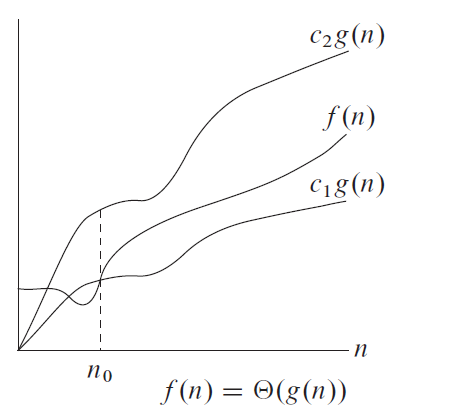
\includegraphics[width=\marginparwidth]{figuras/big-theta}
    \captionof{figure}{{\small{}Interpretación gráfica de la notación 
    asintótica. La notación $f=\Theta(g)$
    implica que $g$ es una cota ajustada para $f$.}}
    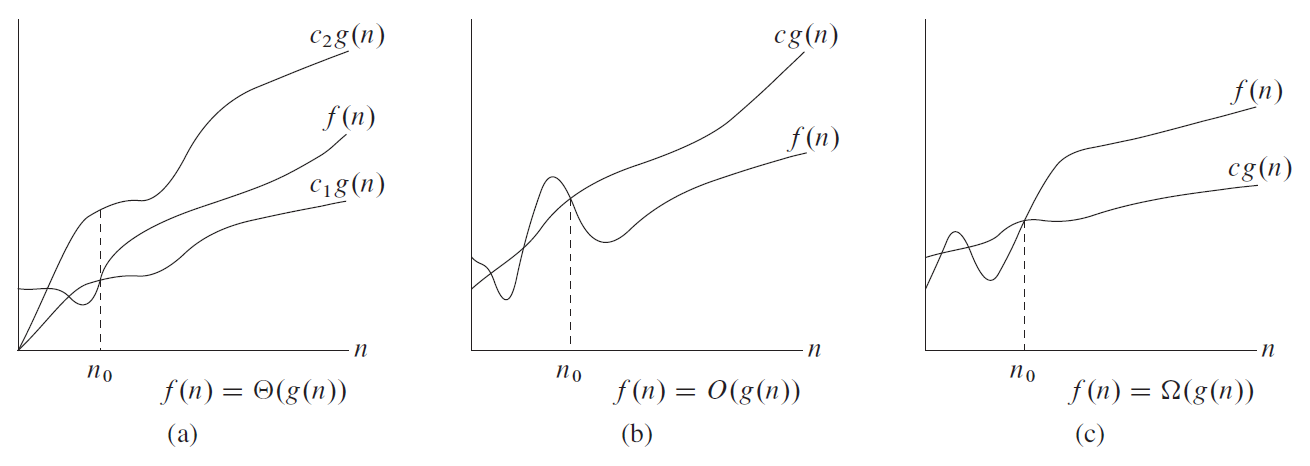
\includegraphics[width=\marginparwidth]{figuras/big-o}
    \captionof{figure}{{\small{}La notación $f=O(g)$
    implica que $g$ es una cota superior para $f$.}}
    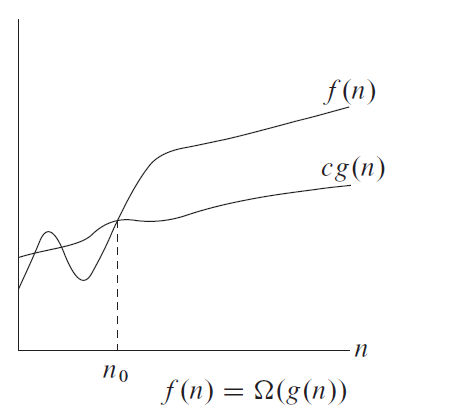
\includegraphics[width=\marginparwidth]{figuras/big-omega}
    \captionof{figure}{{\small{}La notación $f=\Omega(g)$ 
    implica que $g$ es una cota inferior para $f$.}}
}

Sea $n\in\mathbb{N}$ y sean $f:\mathbb{N}\to\mathbb{R}$ y $g:\mathbb{N}\to\mathbb{R}$
dos funciones \emph{asintóticamente positivas}; i.e. $f(n)$ y $g(n)$
siempre son positivos a partir de algún valor de $n$. A continuación
se presentan las definiciones básicas para la notación asintótica.
Obsérvese que, en la notación asintótica, se utiliza el símbolo $=$
en lugar de $\in$ para denotar que una función determinada pertenece
a alguno de los conjuntos introducidos.

\begin{defn}[O grande]
    Denotado como $O(g)$, es el conjunto de todas aquellas funciones
    $f$ para las cuales existen dos constantes $c\in\mathbb{R}$ y $n_{0}\in\mathbb{N}$
    tales que $0\le f(n)\leq c g(n)$, para toda $n\geq n_{0}$. 
\end{defn}

\begin{defn}[$\Omega$ grande]
    Denotado como $\Omega(g)$, es el conjunto de todas aquellas funciones
    $f$ para las cuales existen dos constantes $c$ y $n_{0}$ tales
    que $0\le c g(n)\leq f(n)$, para toda $n\geq n_{0}$.
\end{defn}

\begin{defn}[$\Theta$ grande]
    Denotado como $\Theta(g)$, es el conjunto de todas aquellas funciones
    $f$ para las cuales existen tres constantes $c_{1},c_{2}\in\mathbb{R}$
    y $n_{0}$ tales que $0\le c_{1} g(n)\leq f(n)\leq c_{2} g(n)$,
    para toda $n\geq n_{0}$.
\end{defn}

\begin{prop}
    Se tiene que $f=\Theta(g)$ si y sólo si $f=O(g)$ y $f=\Omega(g)$.
\end{prop}

\begin{defn}[o chica]
    Denotado como $o(g)$, es el conjunto de todas aquellas funciones
    $f$ tales que, para toda constante $c$, existe una constante $n_{0}$
    tal que $0\leq f(n)<c g(n)$ para toda $n\geq n_{0}$.
\end{defn}

\begin{defn}[$\omega$ chica]
    Denotado como $\omega(g)$, es el conjunto de todas aquellas funciones
    $f$ tales que, para toda constante $c$, existe una constante $n_{0}$
    tal que $0\leq c g(n)<f(n)$ para toda $n\geq n_{0}$.
\end{defn}

\begin{prop}
    Si $f=o(g)$, entonces $f=O(g)$.
\end{prop}

\begin{prop}
    Si $f=\omega(g)$, entonces $f=\Omega(g)$.
\end{prop}

\section{Definiciones a partir de límites}

La notación asintótica también se puede definir en términos del límite
de la razón de las funciones involucradas (suponiendo que dicho límite
existe). 

\begin{prop}
    Se tiene que
    
    \[
        \lim_{n\to\infty}\dfrac{f(n)}{g(n)}\in\begin{cases}
            [0,\infty) & \text{si y sólo si }f=O(g)\\
            (0,\infty] & \text{si y sólo si }f=\Omega(g)\\
            (0,\infty) & \text{si y sólo si }f=\Theta(g)
        \end{cases}
    \]
\end{prop}

\begin{prop}
    Se tiene que

    \[
        \text{si }\lim_{n\to\infty}\dfrac{f(n)}{g(n)}=\begin{cases}
        0 & \text{entonces }f=o(g)\\
        \infty & \text{entonces }f=\omega(g)\\
        1 & \text{entonces }f\sim g
        \end{cases}
    \]
\end{prop}

\begin{prop}
    Si $f\sim g$, entonces $f=\Theta(g)$.
\end{prop}

\section{Ordenes de crecimiento}

La notación asintótica permite clasificar las funciones según su tasa
de crecimiento. Tal clasificación se denomina \emph{orden de crecimiento}
(o, simplemente, \emph{orden}). A continuación se presentan los órdenes
de crecimiento más comunes, listados de aquél que crece más lento
al que crece más rápido.

\begin{enumerate}
    \item \emph{Constantes}: $O(1)$
    \item \emph{Logarítmicos}: $O(\log n)$
    \item \emph{Radicales}: $O(\sqrt{n})$
    \item \emph{Lineales}: $O(n)$
    \item \emph{Súper lineales}: $O(n\log n)$
    \item \emph{Cuadráticos}: $O(n^{2})$
    \item \emph{Cúbicos}: $O(n^{3})$
    \item \emph{Exponenciales}: $O(2^{n})$
    \item \emph{Factoriales}: $O(n!)$
\end{enumerate}

Se debe tener cuidado sobre cómo interpretar la lista anterior, ya
que la notación asintótica puede ocultar constantes muy grandes y 
dejar una impresión equivocada de la tasa de crecimiento
de una función comparada con otra. 
Por ejemplo, supóngase que se tiene que $f(n)=10^{100}n=O(n)$
y que $g(n)=10n\cdot\log n=O(n\log n)$. A pesar de que la notación
asintótica indica que $g$ crece más rápido que $f$, en realidad
se trata de lo opuesto, porque la constante $10^{100}$ supera por mucho 
la tasa de crecimiento de $g$.

\begin{thm}
    Sea $k\in\mathbb{N}_{0}$ una constante. Todo polinomio de grado $k$
    pertenece a $\Theta(n^{k})$.
\end{thm}

\begin{proof}
    Sea $f(n)=a_{k}n^{k}+a_{k-1}n^{k-1}+\dots+a_{1}n+a_{0}$ un polinomio
    arbitrario, donde $a_k,\dots,a_{0}\in\mathbb{R}$ son constantes.
    Por la definición de $\Theta$ grande, se requiere demostrar que $f=O(n^{k})$
    y que $f=\Omega(n^{k})$. 
    
    Para demostrar que $f=O(n^{k})$, se tiene que 
    
    \begin{align*}
        a_{k}n^{k}+a_{k-1}n^{k-1}+\dots+a_{1}n+a_{0} &= (a_{k}+a_{k-1}/n+\dots+a_{1}/n^{k-1}+a_{0}/n^{k})n^{k}\\
        &\leq(a_{k}+a_{k-1}+\dots+a_{1}+a_{0})n^{k}
    \end{align*}
    lo que se cumple para toda $n\geq1$. Por lo tanto, $f=O(n^{k})$.
    
    Para demostrar que $f=\Omega(n^{k})$, se tiene que 
    
    \[
        (a_{k}+a_{k-1}/n+\dots+a_{1}/n^{k-1}+a_{0}/n^{k})n^{k}\geq n^{k}
    \]
    lo que se cumple para toda $n\geq1$. Por lo tanto, $f=\Omega(n^{k})$.
\end{proof}

\begin{thm}
    Toda función polinomial crece más rápido que cualquier función logarítmica y
    toda función exponencial crece más rápido que cualquier función polinomial.
    Esto es, sean $k,q\in\mathbb{N}$ constantes, se tiene que $(\log n)^k=o(n^q)$
    y $n^k=o((1+q)^n)$.
\end{thm}

\begin{proof}
    Ambas relaciones se pueden demostrar utilizando límites y la regla
    de L'Hopital. Así, para la primera expresión, se tiene que
    
    \begin{align*}
        \lim_{n\to\infty}\dfrac{(\ln n)^{k}}{n^{q}} &= \left(\lim_{n\to\infty}\dfrac{\ln n}{n^{q/k}}\right)^{k}\\
        &\overset{\text{H}}{=}\left(\lim_{n\to\infty}\dfrac{1/n}{(q/k)n^{q/k-1}}\right)^{k}\\
        &= \left(\lim_{n\to\infty}\dfrac{1}{(q/k)n^{q/k}}\right)^{k}\\
        &= 0
    \end{align*}
    Por lo tanto, $(\log n)^{k}=o(n^{q})$.
    
    Para la segunda expresión, se tiene que 
    
    \begin{align*}
    \lim_{n\to\infty}\dfrac{n^{k}}{(1+q)^{n}} &= \left(\lim_{n\to\infty}\dfrac{n}{(1+q)^{n/k}}\right)^{k}\\
    &\overset{\text{H}}{=}\left(\lim_{n\to\infty}\dfrac{1}{(n/k)(1+q)^{n/k-1}}\right)^{k}\\
    &= 0
    \end{align*}
    Por lo tanto, $n^{k}=o((1+q)^{n})$.
\end{proof}

\section{Propiedades aritméticas}

A continuación se describe cómo hacer aritmética con la notación asintótica.

\subsection{Adición}

La suma de las cotas de dos funciones está gobernada por la función
dominante.

\[
\begin{aligned}
    O(f)+O(g) &= O(\max\{f,g\})\\
    \Omega(f)+\Omega(g) &= \Omega(\max\{f,g\})\\
    \Theta(f)+\Theta(g) &= \Theta(\max\{f,g\})\\
    o(f)+o(g) &= o(\max\{f,g\})\\
    \omega(f)+\omega(g) &= \omega(\max\{f,g\})
\end{aligned}
\]

\subsection{Multiplicación}

La multiplicación de una función con una constante no afecta el comportamiento
asintótico de dicha función.

\[
\begin{aligned}
    O(c f) &= O(f)\\
    \Omega(c f) &= \Omega(f)\\
    \Theta(c f) &= \Theta(f)\\
    o(c f) &= o(f)\\
    \omega(c f) &= \omega(f)
\end{aligned}
\]

Cuando dos funciones se multiplican, ambas contribuyen por igual al
comportamiento asintótico de la función resultante.

\[
\begin{aligned}
    O(f)\cdot O(g) &= O(f\cdot g)\\
    \Omega(f)\cdot\Omega(g) &= \Omega(f\cdot g)\\
    \Theta(f)\cdot\Theta(g) &= \Theta(f\cdot g)\\
    o(f)\cdot o(g) &= o(f\cdot g)\\
    \omega(f)\cdot\omega(g) &= \omega(f\cdot g)
\end{aligned}
\]


\section{Comparación de funciones}

La notación asintótica se puede utilizar como un esquema para comparar
dos funciones, similar a como se puede hacer con números reales. Una
forma intuitiva de verlo es trazando las sig. analogías:

\begin{center}
\begin{tabular}{cc}
    \toprule 
        Números reales & Notación asintótica\tabularnewline
    \midrule
        $a\leq b$ & $f=O(g)$\tabularnewline
        $a\ge b$ & $f=\Omega(g)$\tabularnewline
        $a=b$ & $f=\Theta(g)$\tabularnewline
        $a<b$ & $f=o(g)$\tabularnewline
        $a>b$ & $f=\omega(g)$\tabularnewline
    \bottomrule
\end{tabular}
\par\end{center}

\subsection{Transitividad}

Sea $h:\mathbb{N}\to\mathbb{R}$ una función asintóticamente positiva. 

\begin{itemize}
    \item Si $f=\Theta(g)$ y $g=\Theta(h)$, entonces $f=\Theta(h)$.
    \item Si $f=O(g)$ y $g=O(h)$, entonces $f=O(h)$. 
    \item Si $f=\Omega(g)$ y $g=\Omega(h)$, entonces $f=\Omega(h)$.
    \item Si $f=o(g)$ y $g=o(h)$, entonces $f=o(h)$.
    \item Si $f=\omega(g)$ y $g=\omega(h)$, entonces $f=\omega(h)$.
\end{itemize}

\subsection{Reflexividad}

Las sig. igualdades se satisfacen porque $f(n)=f(n)$ para toda $n$:

\[
    \begin{aligned}
        f &= \Theta(f)\\
        f &= O(f)\\
        f &= \Omega(f)
    \end{aligned}
\]


\subsection{Simetría y simetría traspuesta}

\begin{itemize}
    \item $f=\Theta(g)$ si y sólo si $g=\Theta(f)$.
    \item $f=O(g)$ si y sólo si $g=\Omega(f)$.
    \item $f=o(g)$ si y sólo si $g=\omega(f)$.
\end{itemize}

\subsection{Carencia de tricotomía}

La tricotomía es la propiedad de los números reales donde, dados dos
números $a$ y $b$, siempre se cumple exactamente una de las sig.
condiciones: $a<b$, $a=b$ o $a>b$. La notación asintótica carece
de esta propiedad, pues se puede dar el caso donde no se cumple
que $f=O(g)$ ni que $f=\Omega(g)$. Por ejemplo, si $f(n)$ oscila
periódicamente en lugar de siempre mantener una tendencia a la alza
o a la baja.

\section*{Notas bibliográficas}

Material consultado:
\begin{itemize}
    \item \textcite{cormen_introduction_2009}, págs. 43-52.
    \item \textcite{skiena_algorithm_2012}, págs. 34-41.
    \item \textcite{goodrich_algorithm_2001}, págs. 13-20.
    \item \textcite{baker_2013}
    \item \textcite{leighton_and_rubinfeld_2004}
    \item \textcite{tomescu_2014}
\end{itemize}
